\begin{figure}[H] \centering
\subsection{BDD (SK)}
{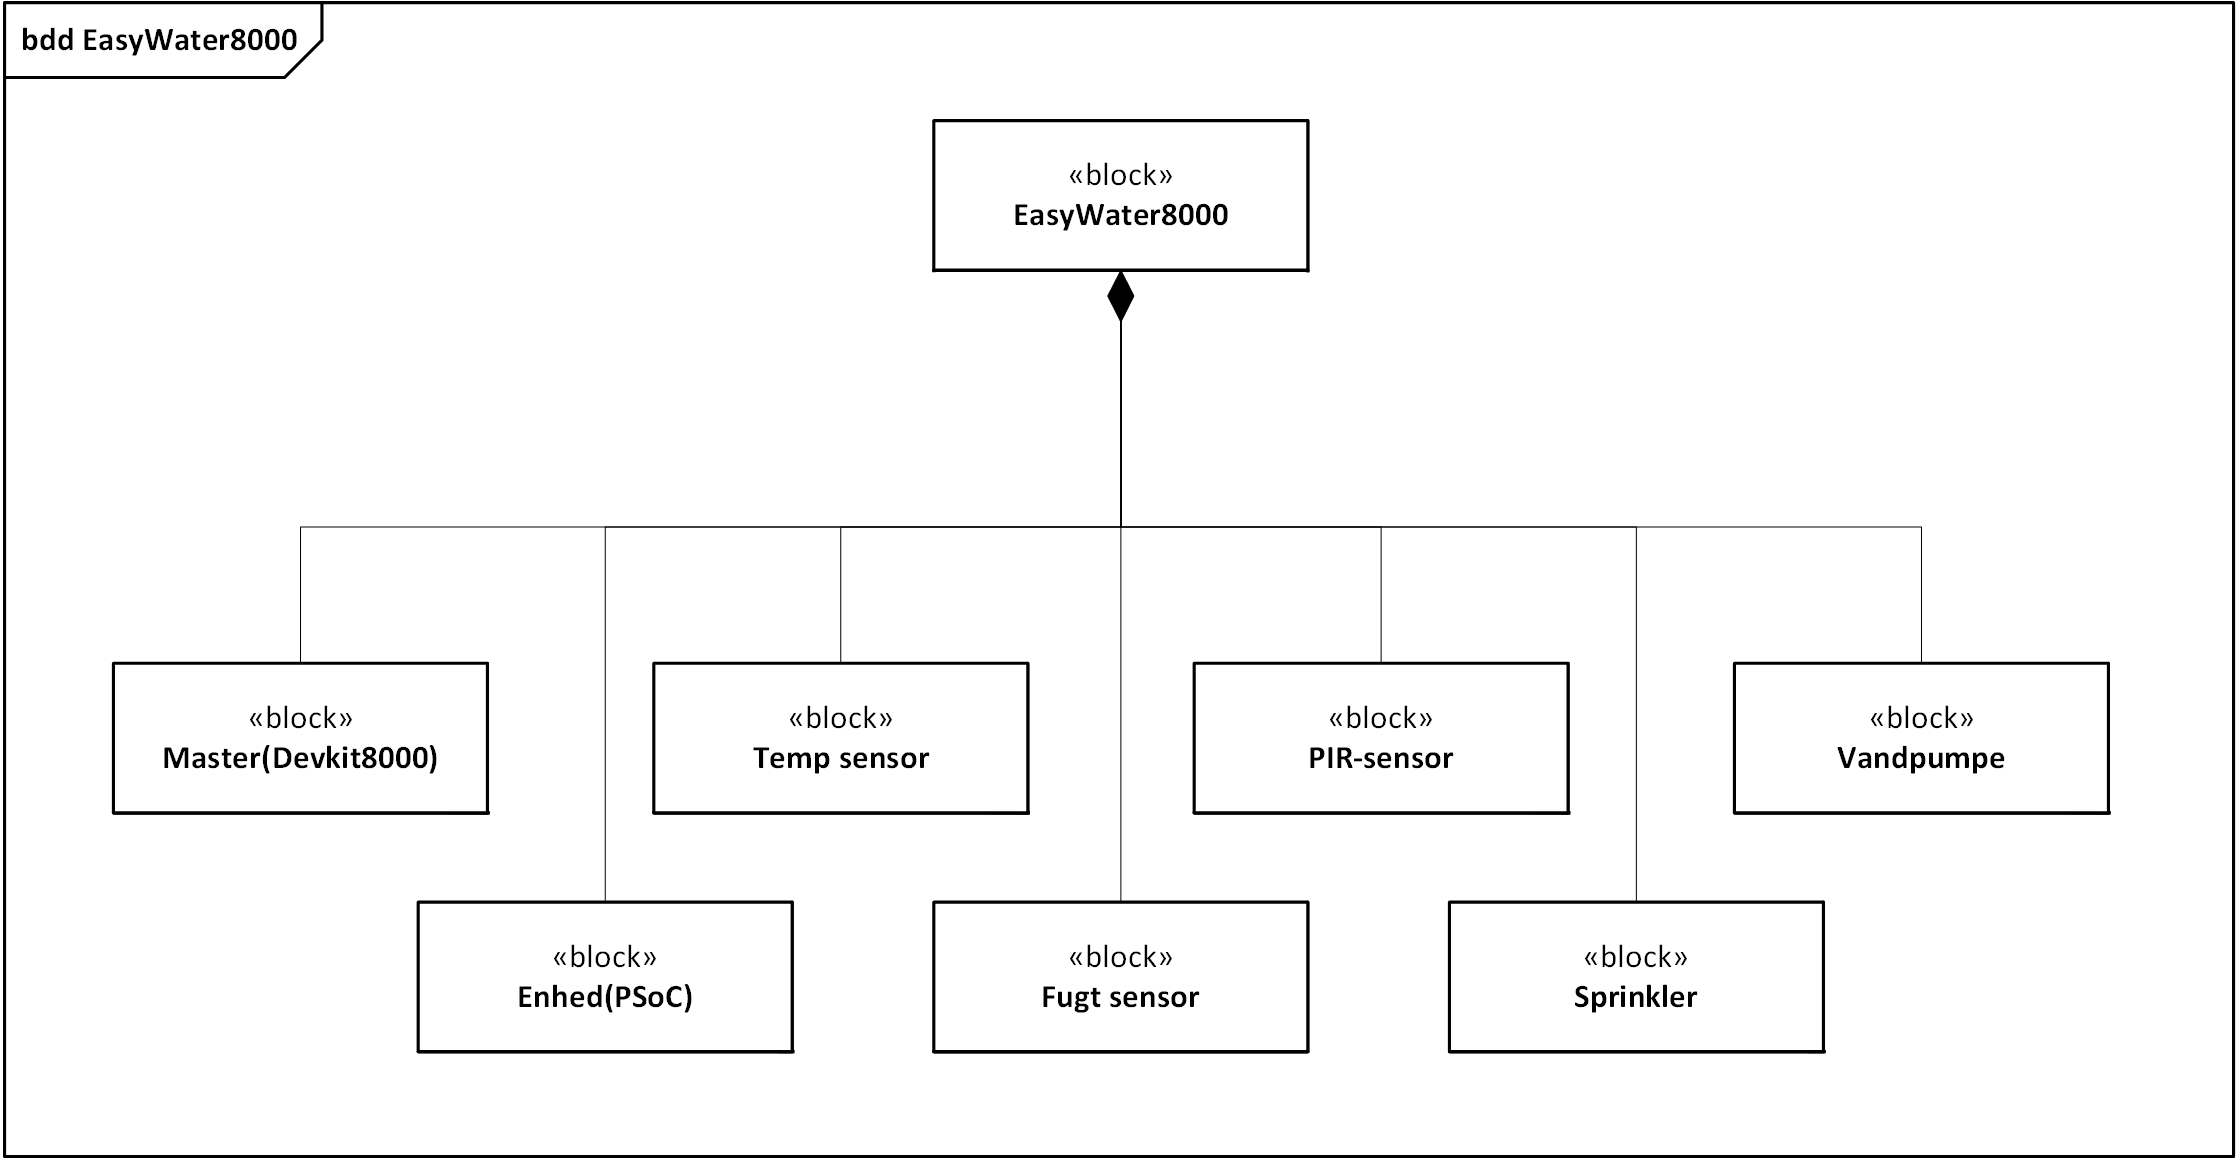
\includegraphics[width=0.9\textwidth]{filer/systemarkitektur/BDD}}
\caption{BDD}
\label{lab:bdd}
\raggedright
\end{figure}
BDD diagrammet giver et overblik over hvad det samlede system består af. \newline \newline

\begin{figure}[H] \centering
\subsection{BDD Master (MK)}
{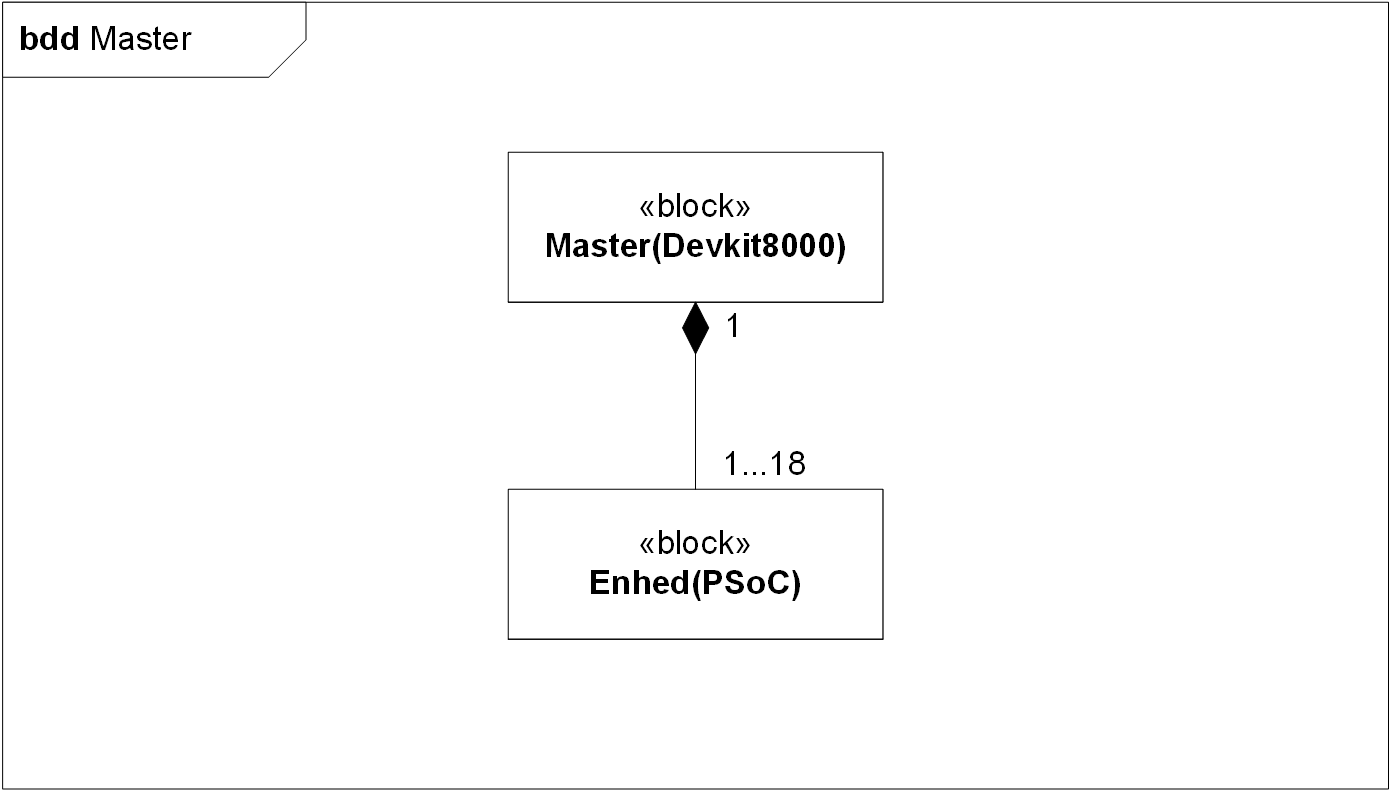
\includegraphics[width=0.9\textwidth]{filer/systemarkitektur/BDD_Master}}
\caption{BDD Master}
\label{lab:bddmaster}
\raggedright
\end{figure}
BDD diagrammet for Master, viser at Master består af et Devkit8000, som kobles op med op til 18 Enheder.

\begin{figure}[H] \centering
\subsection{BDD Enhed (MK)}
{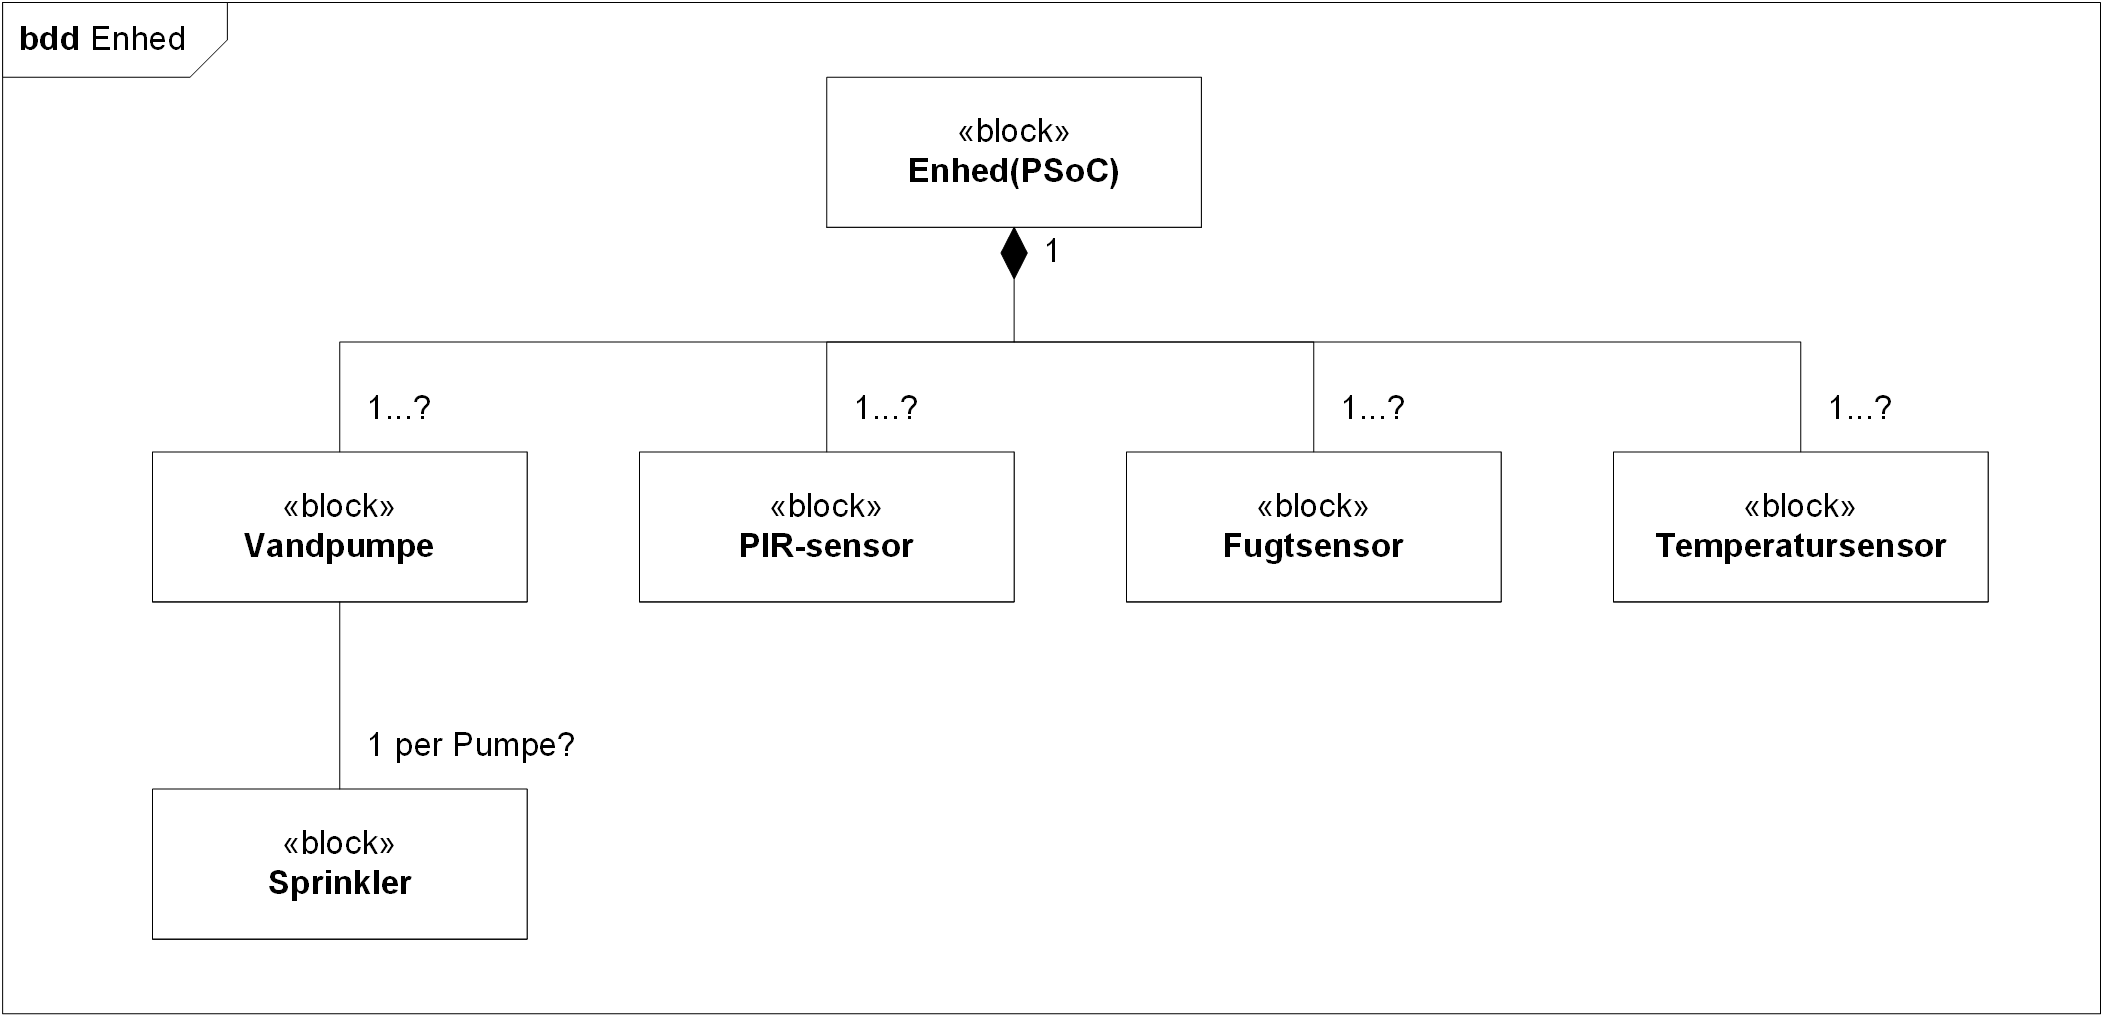
\includegraphics[width=0.9\textwidth]{filer/systemarkitektur/BDD_Enhed}}
\caption{BDD Enhed}
\label{lab:bddenhed}
\raggedright
\end{figure}
BDD diagrammet for Enhed, viser at én Enhed består af én PSoC som kan kobles sammen med op til 20 Vandpumper, 20 Fugtsensorer og 20 Temperatursensorer samt 1 PIR-sensor. Sprinkler bliver i systemet koblet sammen med én Vandpumpe.

\begin{figure}[H] \centering
\subsection{IBD (SK)}
{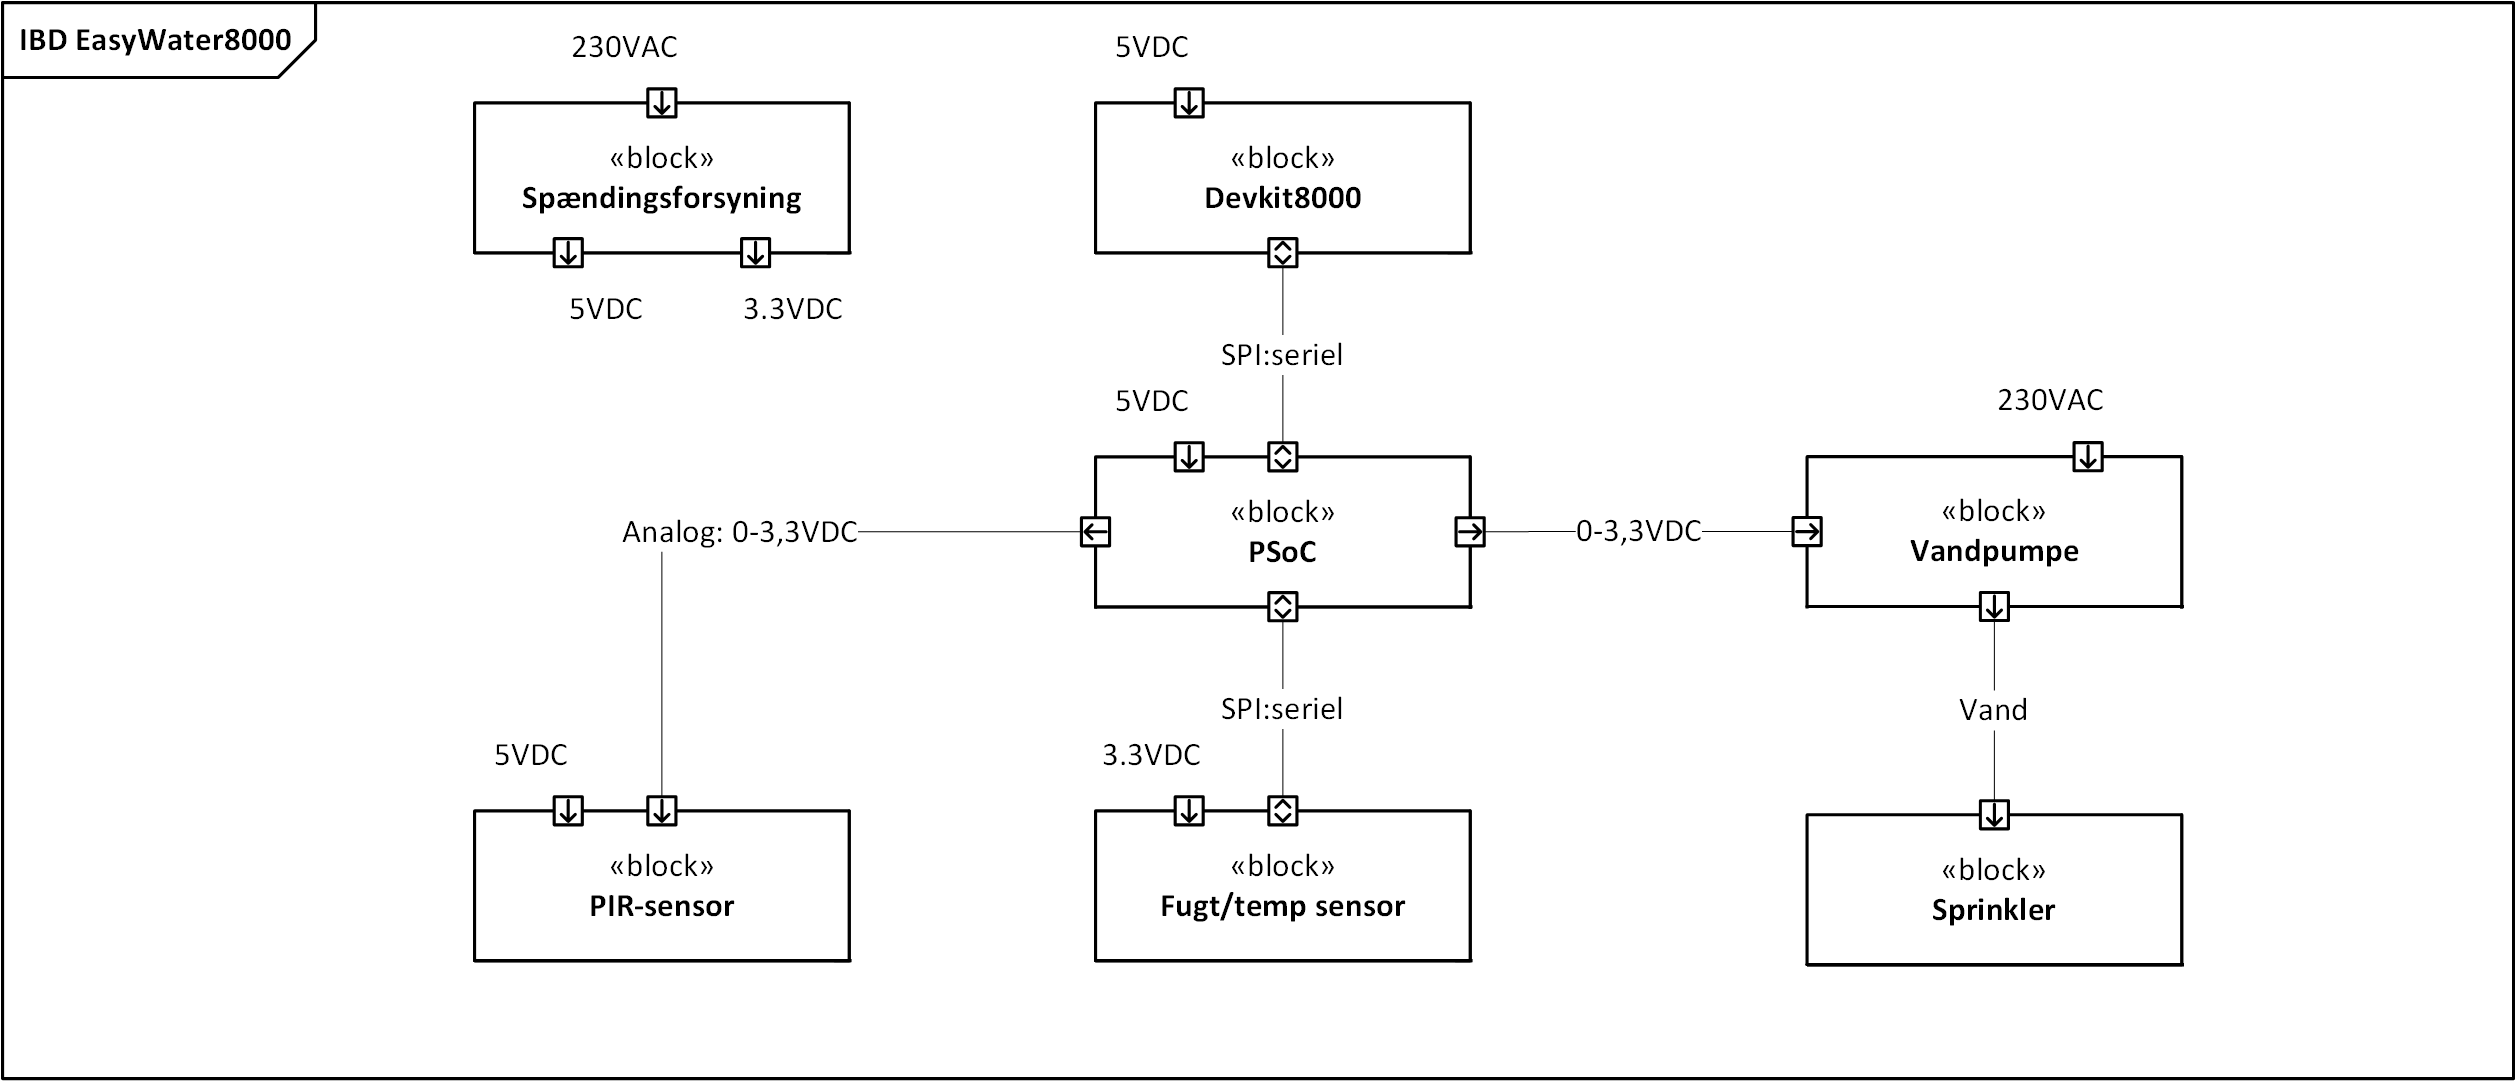
\includegraphics[width=0.9\textwidth]{filer/systemarkitektur/IBD}}
\caption{IBD}
\label{lab:ibd}
\raggedright
\end{figure}
IBD diagrammet giver et internt overblik over hvordan hele systemet er forbundet. Vi ser hvilke type signaler der bliver sendt imellem de forskellige blokke. \newline \newline
\textbf{Spændingsforsyning}: Spændingsforsyningens forbindelser er ikke påtegnet da dette ville give et uoverskueligt diagram, de er i stedet beskrevet med standardflowports.  \newline \newline
\textbf{Integreret fugt- og temperatursensor}: Blokken beskriver at fugt- og temperatursensor er integreret i en chip. \newline \newline

\begin{table}[H] %% Blok og Signal Tabel
\subsection{Grænseflade (HW)}
For at opnå forståelse for signalerne mellem blokkene laves en grænseflade der beskriver de enkelte blokkes porte og hvilke signaler der løber imellem disse.

\subsubsection{Blok beskrivelse (HW)}
Til at beskrive blokkene nærmere er anvendt tabeller som ses herunder. Her er hvert signal i en respektiv blok kommenteret og blokkens funktion er kort beskrevet. 

\caption{Tabel med beskrivelse af respektive blokke}
\begin{small}
\begin{tabular}{|p{3,3cm}|p{3,3cm}|p{3,3cm}|p{3,3cm}|}
\hline
\textbf{Bloknavn} & \textbf{Funktion} & \textbf{Signaler} & \textbf{Kommentar} \\ \hline

Master(Devkit8000) & Styreenhed der modtager input fra touchskærm og kommunikere serielt med Enhed(er) & Touch & Touch \\ \cline{3-4}	
& 				   & SPI & Seriel data kommunikation \\ \hline

Enhed(PSoC) & Enhed er grænsefladen til den fysiske verden igennem sensorer & SPI & Seriel data kommunikation \\ \cline{3-4}
& & TTL 		& Signal fra PIR-sensor	\\ \cline{3-4}
& & TTL 		& Signal til vandpumpe 	\\ \cline{3-4}
& & Analog 	& Signal fra TF-sensor 	\\ \hline

FT-sensor & Måler temperatur og fugt & Analog & Analog signal til Enhed \\ \hline

PIR-sensor & Detektere bevægelse & TTL & Signal til Enhed \\ \hline

Vandpumpe & Forsyner sprinkler med vand & Vand & Vand til Sprinkler \\ \hline
 
Sprinkler & Fordeler vand på golfbane & Vand & Vand til Golfbane \\ \hline

Spændingsforsyning & Forsyner EasyWater8000 & 3,3VDC & Forsyning til FT-sensor \\ \cline{3-4}
& & 5VDC 		& Forsyning til PIR-sensor, Enhed og Master 	\\ \hline
\end{tabular}
\end{small}
\label{table:Bloktabel}
\end{table}

\begin{table}[H]
\subsection{Signal beskrivelse (HW)}
For at fuldende beskrivelsen af grænsefladen er der lavet en signaltabel som kan ses herunder. Hvert signal er beskrevet og tilknyttet en kort kommentar. Området et signal er defineret under, er også beskrevet. Blok og terminal indgår også. 
\caption{Tabel over signaler med terminaler}
\begin{small}
\begin{tabular}{|p{2cm}|p{2cm}|p{2cm}|p{2cm}|p{2cm}|p{2,2cm}|}
\hline

\textbf{Signal-navn}	&\textbf{Funktion} 		&\textbf{Område} &\textbf{Port 1} 	&\textbf{Port 2} 			&\textbf{Kommentar} \\ \hline

SPI 					&Seriel kommunikation 	& 				&Master (DK\_02)		&Enhed (P\_DK)				&					 \\\hline

TTL 					&TTL 					&0\slash3,3V 	&PIR-sensor (PIR\_01) &Enhed (P\_PIR)			&					\\\cline{4-5}
					&						&				&Enhed (P\_VP)		&Vandpumpe (VP\_01)			&					\\\hline
					
Analog				&Analog 					&0-3,3V 			&FT-sensor (FT\_01) &Enhed (P\_FT)			&	    				\\\hline

\end{tabular}
\end{small}
\label{table:Signaltabel}
\end{table}
